\documentclass[conference]{IEEEtran}

\IEEEoverridecommandlockouts
% The preceding line is only needed to identify funding in the first footnote. If that is unneeded, please comment it out.
\usepackage{cite}
\usepackage{amsmath,amssymb,amsfonts}
\usepackage{algorithmic}
\usepackage{graphicx}
\usepackage{textcomp}
\usepackage{xcolor}
\def\BibTeX{{\rm B\kern-.05em{\sc i\kern-.025em b}\kern-.08em
    T\kern-.1667em\lower.7ex\hbox{E}\kern-.125emX}}

\usepackage{enumerate}
\usepackage{color}
\usepackage{xcolor}
\usepackage{listings}
\usepackage{mathtools}
\usepackage{graphicx}
\graphicspath{ {./} }
\usepackage{pgfplots}
\usepackage{capt-of}  % <---
\usepackage{cuted}    % <===
\usepackage{hyperref}
\usepackage{color,soul}
% \usepackage[style=authoryear-comp]{biblatex}

% \bibliography{IEEEexample}

\lstdefinelanguage{RSVAssembler}
{
  alsoletter={.}, % allow dots in keywords
  alsodigit={0x}, % hex numbers are numbers too!
  morekeywords=[1]{ % instructions
    lb, lh, lw, lbu, lhu,
    sb, sh, sw,
    sll, slli, srl, srli, sra, srai,
    add, addi, sub, lui, auipc,
    xor, xori, or, ori, and, andi,
    slt, slti, sltu, sltiu,
    beq, bne, blt, bge, bltu, bgeu,
    j, jr, jal, jalr, ret,
    scall, break, nop
  },
  morekeywords=[2]{ % sections of our code and other directives
    .align, .ascii, .asciiz, .byte, .data, .double, .extern,
    .float, .globl, .half, .kdata, .ktext, .set, .space, .text, .word
  },
  morekeywords=[3]{ % registers
    zero, ra, sp, gp, tp, s0, fp,
    t0, t1, t2, t3, t4, t5, t6,
    s1, s2, s3, s4, s5, s6, s7, s8, s9, s10, s11,
    a0, a1, a2, a3, a4, a5, a6, a7,
    ft0, ft1, ft2, ft3, ft4, ft5, ft6, ft7,
    fs0, fs1, fs2, fs3, fs4, fs5, fs6, fs7, fs8, fs9, fs10, fs11,
    fa0, fa1, fa2, fa3, fa4, fa5, fa6, fa7
  },
  morecomment=[l]{;},   % mark ; as line comment start
  morecomment=[l]{\#},  % as well as # (even though it is unconventional)
  morestring=[b]",      % mark " as string start/end
  morestring=[b]'       % also mark ' as string start/end
}


\lstset{language=Verilog,keywordstyle={\bfseries \color{blue}}}

\definecolor{mygreen}{rgb}{0,0.6,0}
\definecolor{mygray}{rgb}{0.5,0.5,0.5}
\definecolor{mymauve}{rgb}{0.58,0,0.82}
\definecolor{codegreen}{rgb}{0,0.6,0}
\definecolor{codegray}{rgb}{0.5,0.5,0.5}
\definecolor{codepurple}{rgb}{0.58,0,0.82} 
\definecolor{backcolour}{rgb}{0.95,0.95,0.92}


\lstset{ %
  backgroundcolor=\color{white},   % choose the background color
  basicstyle=\footnotesize,        % size of fonts used for the code
  breaklines=true,                 % automatic line breaking only at whitespace
  captionpos=b,                    % sets the caption-position to bottom
  commentstyle=\color{mygreen},    % comment style
  escapeinside={\%*}{*)},          % if you want to add LaTeX within your code
  % morekeywords=[1]{arg,pos},
  keywordstyle=\color{blue},       % keyword style
  stringstyle=\color{mymauve},     % string literal style
  backgroundcolor=\color{backcolour},   
    commentstyle=\color{codegreen},
    keywordstyle=\color{magenta},
    numberstyle=\tiny\color{codegray},
    stringstyle=\color{codepurple},
    basicstyle=\ttfamily\footnotesize,
    breakatwhitespace=false,         
    breaklines=true,                 
    captionpos=b,                    
    keepspaces=true,                 
    numbers=left,                     
    numbersep=5pt,                  
    showspaces=false,                
    showstringspaces=false,
    % keywordstyle=\color{weborange},
    showtabs=false,                  
    tabsize=2
}



\begin{document}


\title{FPGA-based Accelerator for Vector Search\\
% {\footnotesize \textsuperscript{*}Note: Sub-titles are not captured in Xplore and
% should not be used}
% \thanks{Identify applicable funding agency here. If none, delete this.}
}

\author{\IEEEauthorblockN{Sanjay Seshan}
\IEEEauthorblockA{\textit{Electrical Engineering and Computer Science} \\
\textit{Massachusetts Institute of Technology}\\
Cambridge, MA, United States \\
seshan@mit.edu}
\and
\IEEEauthorblockN{Lasya Balachandran}
\IEEEauthorblockA{\textit{Electrical Engineering and Computer Science} \\
\textit{Massachusetts Institute of Technology}\\
Cambridge, MA, United States \\
lasyab@mit.edu}
% \and
% \IEEEauthorblockN{3\textsuperscript{rd} Given Name Surname}
% \IEEEauthorblockA{\textit{dept. name of organization (of Aff.)} \\
% \textit{name of organization (of Aff.)}\\
% City, Country \\
% email address or ORCID}
% \and
% \IEEEauthorblockN{4\textsuperscript{th} Given Name Surname}
% \IEEEauthorblockA{\textit{dept. name of organization (of Aff.)} \\
% \textit{name of organization (of Aff.)}\\
% City, Country \\
% email address or ORCID}
% \and
% \IEEEauthorblockN{5\textsuperscript{th} Given Name Surname}
% \IEEEauthorblockA{\textit{dept. name of organization (of Aff.)} \\
% \textit{name of organization (of Aff.)}\\
% City, Country \\
% email address or ORCID}
% \and
% \IEEEauthorblockN{6\textsuperscript{th} Given Name Surname}
% \IEEEauthorblockA{\textit{dept. name of organization (of Aff.)} \\
% \textit{name of organization (of Aff.)}\\
% City, Country \\
% email address or ORCID}
}

\maketitle
\thispagestyle{plain}
\pagestyle{plain}
\begin{abstract}
With the application of graphs in large-scale modeling, such as social network analysis and image and video segmentation, among other applications, graphs are increasingly being used to encode and find complex relationships between data for machine learning models, leading to an increased need for optimization of these models. As a result, in order to better support model-specific algorithm efficiency, there has been work to create specialized hardware accelerators focusing on aspects such as memory accessing, latency, and resource allocation. However, current accelerators for graph problems are not scalable and can only be optimized for a single application, such as graph random walks or matrix multiplication. Existing systems also run on CPU or GPUs. Following from prior accelerator work on FPGAs, we plan to implement a graph-based vector search algorithm, based on iQAN, that runs on an FPGA produce better algorithm performance than on existing systems and can be used for more versatile applications.


% One way to reduce computation is by graph sampling, where we select a random subset of vertices representative of the entire graph, when traversing the graph from a starting set of nodes, but sampling graphs, or reducing them, is hard to perform efficiently. 

% Due to the reprogrammability of FPGAs and following from previous work on hardware and software co-design for an inverted file index (IVF)-product quantization (PQ)-based vector search algorithm on FPGAs, we propose an FPGA-based accelerator that builds off of the iQAN and graph sampling framework to provide an interface to efficiency search graphs [2]. 
% % This system will work to provide a general interface for graph sampling and pattern search problems. 
% Some applications of this system include graph-based vector search (e.g. iQAN) for machine learning applications and graph pattern mining on the sampled graphs.

% This project will build on the work of iQAN (graph-based vector search) and NextDoor (efficient graph sampling on GPUs) [1, 3]. It is also part of our UROP with Arvind and Xuhao Chen in the Computation Structures Group at CSAIL.

\end{abstract}

\begin{IEEEkeywords}
FPGA, accelerator, graph, vector search
% component, formatting, style, styling, insert
\end{IEEEkeywords}

\section{Introduction}
The goal of this project is to implement an accelerator for a general-use search algorithm. One of the main problems when working with large graphs is the large amount of computations, which is a reason why current accelerators have focused on specific optimizations on CPU or GPU systems \cite{jiang2023co}.  One way we can reduce computations is by running the calculations on only a subset of the graph. For example, the novel graph-based vector search algorithm iQAN \cite{peng2023iqan} uses a priority queue of certain length to approximate the most similar points and avoid brute-force-checking all of the points. Graph sampling, where we select a random subset of vertices representative of the entire graph, can also be used to reduce a graph. We are planning to implement a vector search algorithm on an FPGA to get improved results as a result of higher customizability with pipelining, parallelizing, and optimizing the architecture.

The following sections will discuss the implementation of our system and individual components of the system. As this document is a preliminary report, we will focus on the parts that have been completed. We have built large portions of the base components of our system and verified their accuracy against custom test benches.

\section{System Overview}
Based on the paper on iQAN \cite{peng2023iqan}, we are implementing the Best First Search (BFiS), a graph-based vector search algorithm, on the FPGA. The algorithm is as follows:

\begin{lstlisting}[language=c]
Input: graph G, starting point P, query Q, queue capacity L
Output: K nearest neighbors of Q
priority queue S <- {} /* sorted based on distance */
index i <- 0
compute dist(P, Q)
add P into S
while S has unchecked vertices do /* stop condition */
    i <- the index of the 1st unchecked vertex in S
    mark v_i as checked
    foreach neighbor u of v_i in G do
        if u is not visited then
            mark u as visited
            compute dist(u,Q)
            add u into S /* u is unchecked */
    if S.size() > L then S.resize(L)
return the first K vertices in S
\end{lstlisting}




Our design [Figure \ref{fig:blockdiagram}] is composed of three main components: graph storage, vector search, and SPI output. The vector search module is a much larger module that is composed of several different modules.

% INSERT BLOCK DIAGRAM
\begin{figure}[htbp]
% \lipsum[1]
\begin{strip} % <--- defined in "cuted"
\centerline{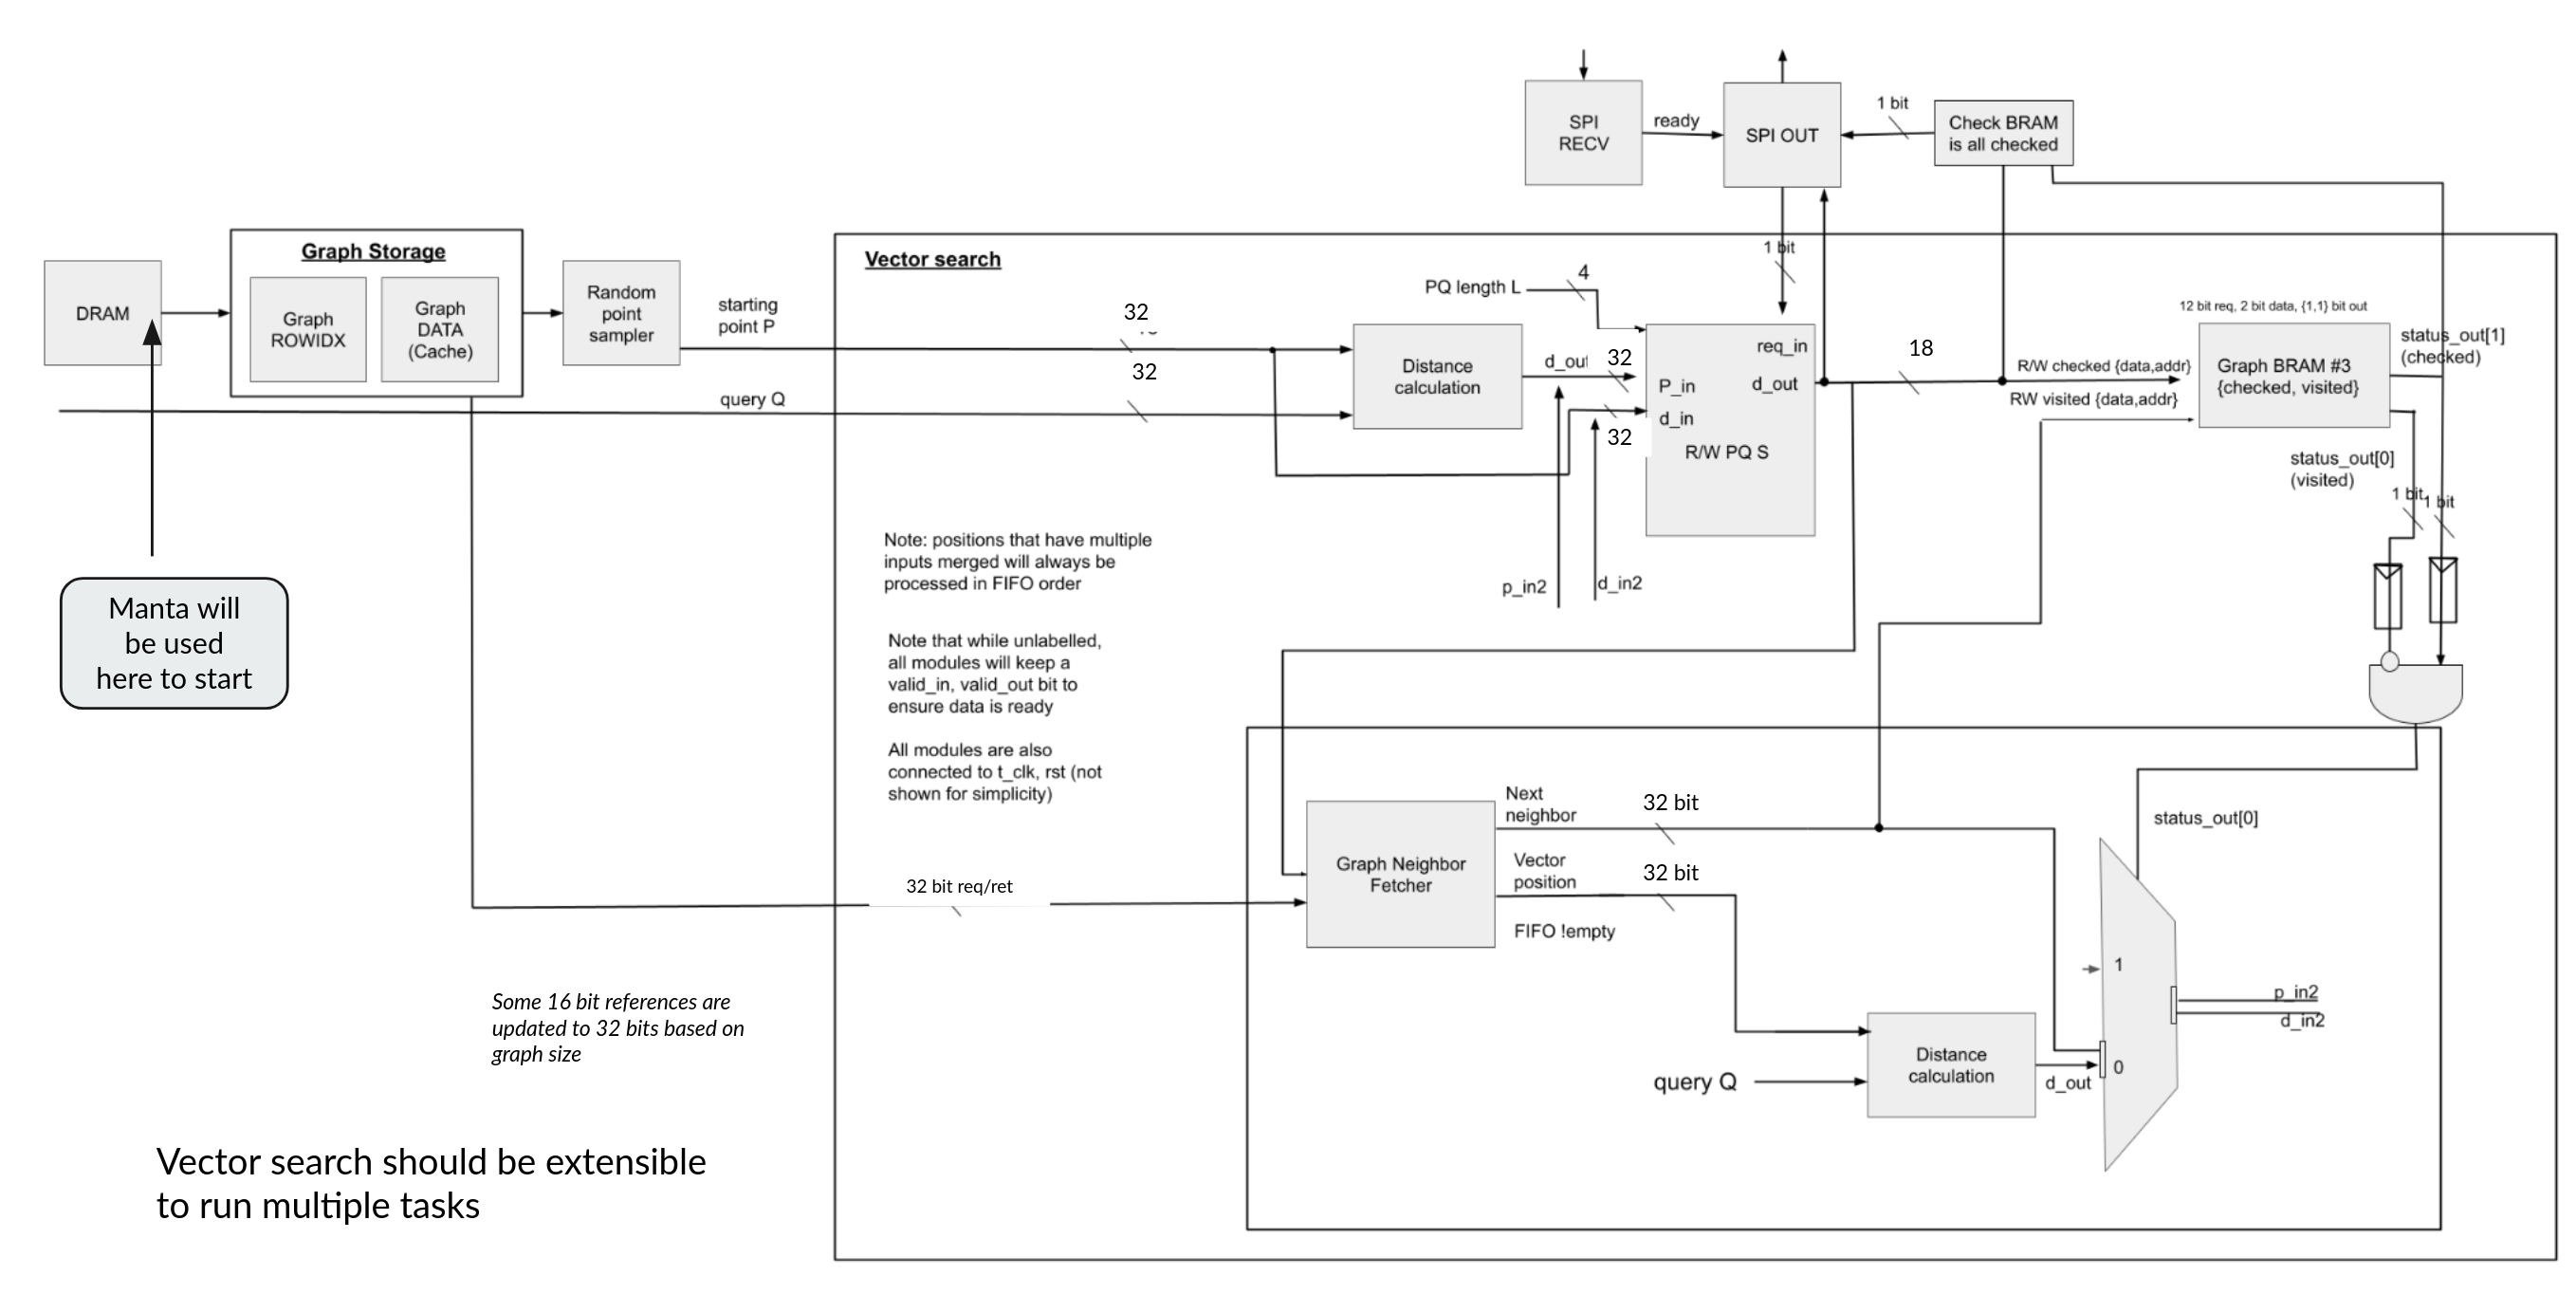
\includegraphics[width=\linewidth]{block.png}}
\caption{Full block diagram of our system.}
\label{fig:blockdiagram}
\end{strip}
    
% \lipsum[2-15]
\end{figure}

We have chosen to implement our system in a bottom-up approach, implementing core features such as queues, priority queues, memory interfaces, and related layouts before designing the interconnections for each module.

\section{CPU Implementation}

\subsection{Design}

We have created a basic implementation of BFiS in C++. The code can be found in Appendix section \ref{sssec:cpucode}.
By default, priority queues in C++ have a max heap structure (can be converted to min heap), where only the first element can be accessed or removed from the queue. Since, according to the BFiS pseudocode, we must be able to access the closest visited point  that we have not yet checked in the priority queue, we created two priority queues: a min heap \texttt{S} to keep track of all visited points and a max heap \texttt{checked} to keep track of checked points. 

In our min heap structure, our top point is our closest unchecked point. Once we check a point in \texttt{S}, we add it to \texttt{checked} if either the size of \texttt{checked} is less than our desired priority queue capacity \texttt{L} or the distance from the query to the point is less than the distance of the query to the top point in \texttt{checked} (farthest checked point from the query). If the size of \texttt{checked} is greater than \texttt{L} after adding a point, we pop the top element off of the queue, allowing us to maintain queue capacity \texttt{L}. 

We exit the \texttt{while} loop when the capacity of \texttt{checked} is \texttt{L} and the closest point in \texttt{S} is farther than the farthest point in \texttt{checked} since this denotes that the \texttt{L} closest points (based on our approximation) have all been checked. We then returned the bottom \texttt{k} elements in \texttt{checked} to represent the approximate \texttt{k} closest points to the query.

We want to design the system on the FPGA such that it is similar to this CPU design. For example, since we can access and remove the top element of priority queue \texttt{S} and access its size, we aim for our priority queue module to have similar capabilities.

\subsection{Verification and Performance}

The C++ implementation of BFiS was tested against a data set containing 10,000 points of 128 dimensions each and 100 queries. Table \ref{tab:cpu} shows the algorithm performance in terms of accuracy and runtime with varying sizes of \texttt{L} and \texttt{k}$=100$. The accuracy was compared to the actual \texttt{k} closest points from a brute force approach. A C++ implementation of the brute force approach runs in about 0.8 seconds.

\begin{table}[hbt!]
\caption{Performance of BFiS (C++) on graph with 10,000 points}
\label{tab:cpu}
\resizebox{\columnwidth}{!}{%
\begin{tabular}{|c|c|c|}
\hline
\textbf{PQ Capacity L} & \textbf{Accuracy} & \textbf{Runtime (sec)} \\ \hline
\textbf{200}           & 0.8434            & 0.072317               \\ \hline
\textbf{500}           & 0.9482            & 0.121287               \\ \hline
\textbf{700}           & 0.9892            & 0.144219               \\ \hline
\textbf{900}           & 0.9893            & 0.163350               \\ \hline
\textbf{1000}          & 0.9993            & 0.172315               \\ \hline
\end{tabular}%
}
\end{table}

Based on the accuracies, the algorithm seems to approximate the \texttt{k} closest points well. As the size of \texttt{L} increases, the accuracy of the approximation approaches 1 since the algorithm visits more points. The runtime of BFiS is also significantly faster than the runtime of the brute force approach and will be used a baseline comparison with our accelerator. We plan on further testing the CPU implementation with graphs of up to 1,000,000 points for eventual comparison with our FPGA version, but for the scope of this project, we will not be using graphs that large.

% This measurement 
% and others are deliberate, using specifications that anticipate your paper 
% as one part of the entire proceedings, and not as an independent document. 
% Please do not revise any of the current designations.

\section{Completed Core components}

\subsection{Distance Calculator}

We implemented a distance calculator that computes the square of the Euclidean distance between two points, according to the following equations:

$$\text{dist}(\vec v) = ||\vec v||$$
$$=\text{dist}(x_1,y_1,x_2,y_2+\dots)=\sqrt{(x_1-y_1)^2+(x_2-y_2)^2+\dots}$$
$$\text{dist}^2(x_1,y_1,x_2,y_2,\dots)=(x_1-y_1)^2+(x_2-y_2)^2+\dots$$


To avoid implementing a square root, we decided to consider the square of the distance anywhere dist is used since this calculation will provide the same result to our algorithm.


The input vertex and query to our distance module represent two vectors (a point in the graph and the query), each of dimension DIM, which is set at compile time. Our graph fetcher module (Section \ref{sssec:graphfetcher}) provides the position vector of the vertex, while our query is an input to the system. Each element of the vertex is provided sequentially on subsequent cycles (i.e. $P_0$ and $Q_0$ on the first cycle, $P_1$, $Q_1$ on the second cycle, etc). We assume that the elements of the input vectors are in order in memory for all practical purposes. 

\begin{lstlisting}[language=Verilog]
module distance #(parameter DIM = 2)(
  input wire clk_in,
  input wire rst_in,
  input wire data_valid_in [DIM-1:0],
  input wire [31:0] vertex_pos_in [DIM-1:0],
  input wire [31:0] query_pos_in [DIM-1:0],
  output logic [31:0] distance_sq_out,
  output logic data_valid_out
  );
\end{lstlisting}

This system is pipelined using a state machine with two states: one to subtract and multiply and another to recursively add the squares of differences, as shown in Figure \ref{fig:distfig}. On the first cycle, we calculate $Q_0 - P_0$ and on the second cycle, we calculate square the result. On the second cycle, we also calculate $Q_1 - P_1$ and similarly parallelize our subtraction and multiplication on future cycles. Overall, this state takes $DIM+1$ cycles. Once we have finished squaring all the differences, we merge the squares, or add them together, to get the final result. Our recursive adder takes 2 cycles.
% This system is fully pipelined and reads inputs as they arrive, which we assume are in order in memory for all practical purposes.

\begin{figure}[htbp]
\centerline{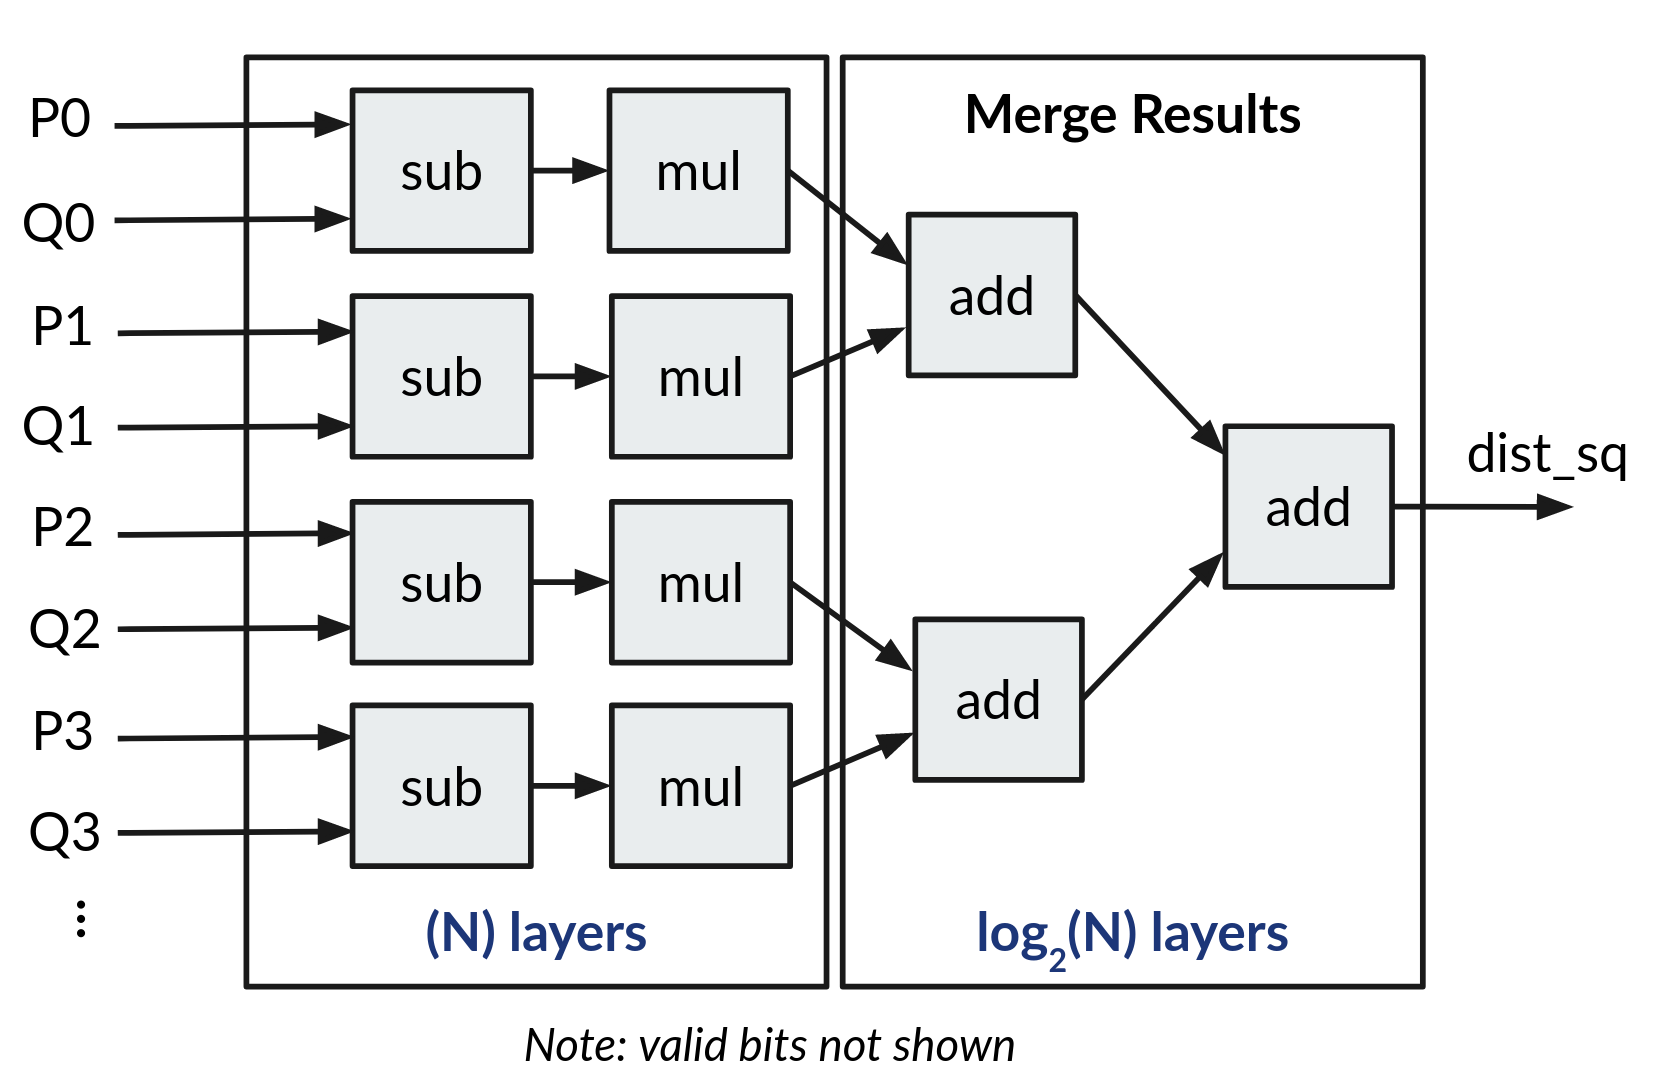
\includegraphics[width=8cm]{dist.png}}
\caption{Distance calculator tree. }
\label{fig:distfig}
\end{figure}

We created a testbench to simulate our distance calculator with dimensions 3, 4, and 9. Our module correctly returned the square of the distances for each with 6, 7, and 12 cycles, respectively.
% For DIM=3, query (18, 97, 45) and vertex (980, 89, 12), our module correctly returned 926597 in 6 cycles. For DIM=4, query (5, 7, 10, 50), and vertex (8, 2, 15, 80), our module correctly returned 959 in 7 cycles. For DIM=9, query (23, 67, 2, 99, 17, 103, 1, 53, 18), and vertex (89, 123, 231, 82, 7, 12, 20, 39, 19), our module correctly returned 69161 in 12 cycles.

% \begin{lstlisting}[language=Verilog]
% module distance #(parameter DIM = 2)(
%   input wire clk_in,
%   input wire rst_in,
%   input wire data_valid_in [DIM-1:0],
%   input wire [31:0] vertex_pos_in [DIM-1:0],
%   input wire [31:0] query_pos_in [DIM-1:0],
%   output logic [31:0] distance_sq_out,
%   output logic data_valid_out
%   );
% \end{lstlisting}


\subsection{FIFO Queues}

We developed an effective FIFO [Figure \ref{fifofig}] that is versatile for use throughout our system. This FIFO is important for maintaining ordering for memory requests, buffering outputs, buffering inputs for distance calculations, and more. 

We provide an easy interface for our FIFOs:
\begin{lstlisting}[language=Verilog]
module FIFO #(parameter DATA_WIDTH = 32, parameter DEPTH = 8)(
  input wire clk_in,
  input wire rst_in,
  input wire deq_in,
  input wire [DATA_WIDTH-1:0] enq_data_in,
  input wire enq_in,
  output logic full_out,
  output logic [DATA_WIDTH-1:0] data_out,
  output logic empty_out,
  output logic valid_out
);
\end{lstlisting}

% INSERT FIFO DIAGRAM
\begin{figure}[htbp]
\centerline{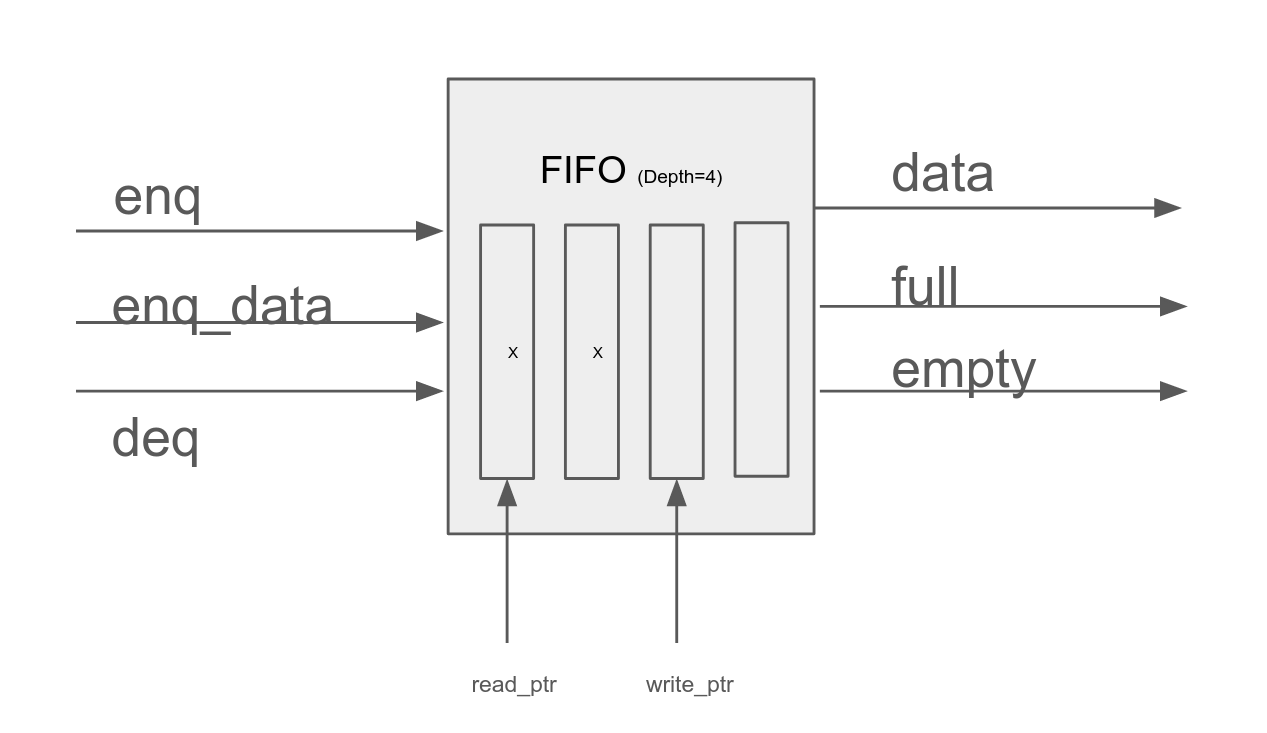
\includegraphics[width=8cm]{fifo.png}}
\caption{Core FIFO Implementation}
\label{fifofig}
\end{figure}
Our FIFO consists of four main components -- the queue array, a read pointer, a write pointer, and an array of valid bits. The FIFO is fixed size and is allocated a depth and width at initialization. The read pointer gets incremented upon dequeueing and the write pointer gets incremented upon enqueueing. Pointers wrap around when reaching the maximum depth of the queue, assuming it is not full. The valid bits are used to determine if the queue is full or empty, on the condition that the read and write pointers are at the same location. Such a queue allows us to effectively buffer all inputs and outputs to our system, making pipelining easier.

We created a testbench enqueuing and dequeuing elements from the FIFO to verify that it is working. Enqueing and dequeuing elements takes 1 cycle each.

\subsection{Priority Queue}

Our priority queue [Figure \ref{pqfig}] is effectively implemented as a searchable FIFO that functions as a min heap. We have a data array, which contains the vertex ID, and a tag array, which contains the corresponding distances. Elements are dequeued in increasing order in the tag array. At each cycle, we identify the smallest tag in the tag array combinationally by comparing all the elements in the array.

A FIFO is used to maintain the least recently used (LRU) ordering in the cache, so that we can insert elements to only empty slots in the priority queue array(s). The LRU FIFO is largely the same as a regular FIFO but allows synchronous dequeueing (i.e. can read and dequeue in the same cycle) and preinitializing values in order. The preinitialized values correspond to each empty index in the priority queue array. Dequeueing from this FIFO allows a quick identification of empty positions and a way to easily recycle positions, once dequeued from the priority queue. The smallest tag and its associated data are returned on dequeue and its index is freed in the LRU FIFO.

\begin{figure}[htbp]
\centerline{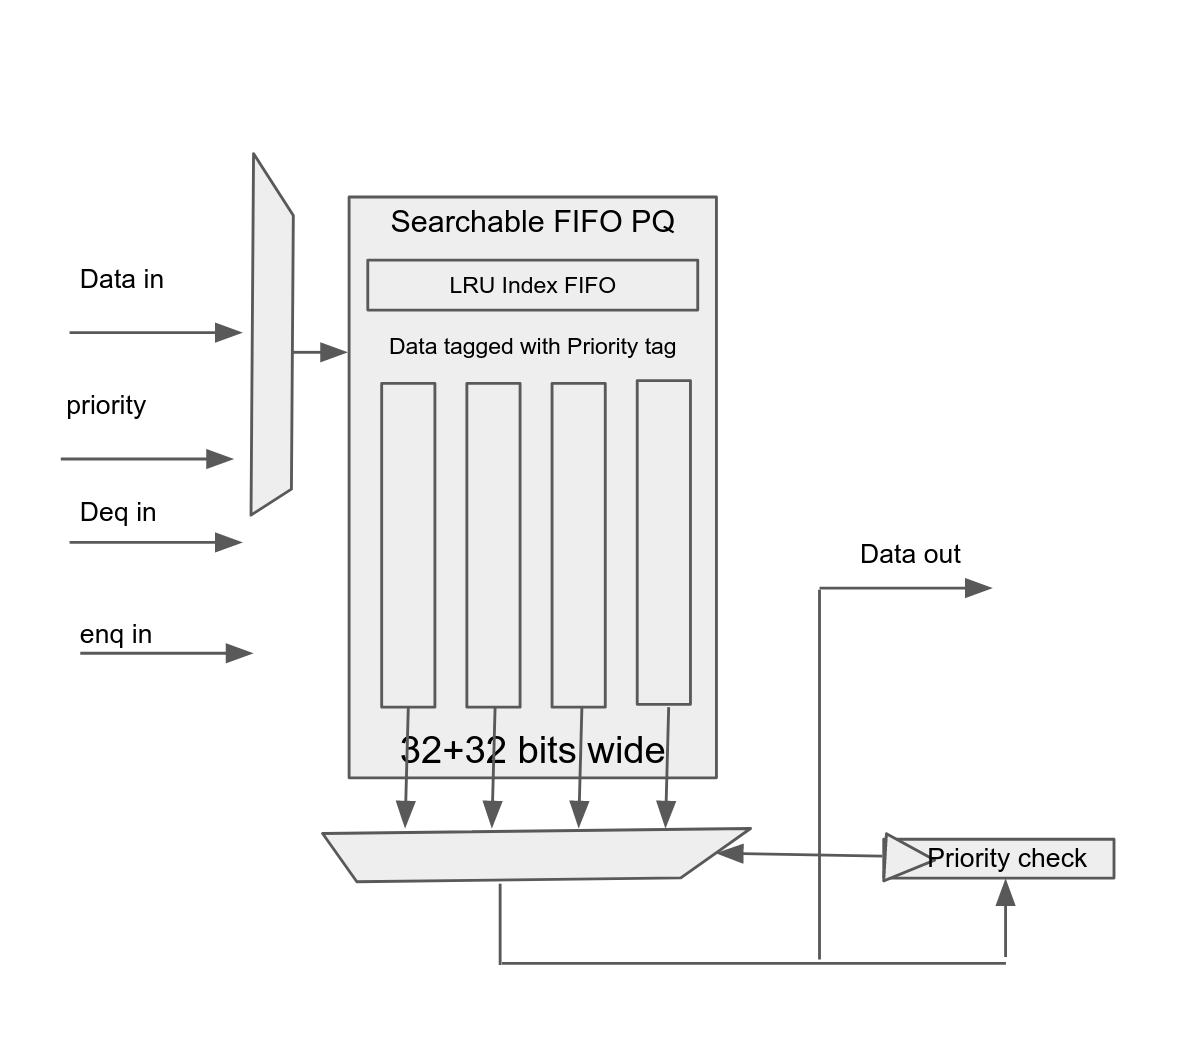
\includegraphics[width=8cm]{pq.png}}
\caption{Implemented Priority Queue using a Searchable FIFO.}
\label{pqfig}
\end{figure}


We provide a simple interface for a priority queue that is similar to a FIFO, but allows tagging entries with a distance.
\begin{lstlisting}[language=Verilog]
module PriorityQueue #(parameter DATA_WIDTH = 32, parameter TAG_WIDTH = 32, parameter DEPTH = 8)(
  input wire clk_in,
  input wire rst_in,
  input wire deq_in,
  input wire [DATA_WIDTH-1:0] enq_data_in,
  input wire [TAG_WIDTH-1:0] enq_tag_in,
  input wire enq_in,
  output logic full_out,
  output logic [DATA_WIDTH-1:0] data_out,
  output logic [TAG_WIDTH-1:0] tag_out,
  output logic [$clog2(DEPTH):0] size_out,
  output logic empty_out,
  output logic valid_out
);
\end{lstlisting}

We will try to improve its performance using other structures in the coming weeks.

We tested our priority queue by enqueuing a set of inputs and verifying that the system dequeues the inputs in increasing order of tag. Enqueuing and dequeuing elements takes 1 cycle each.

\subsection{General Memory Storage}

Our Memory storage is two BRAMs right now [Figure \ref{csrfig}], containing the graph in CSR format.

% CSR TABLE HERE
\begin{figure}[htbp]
\centerline{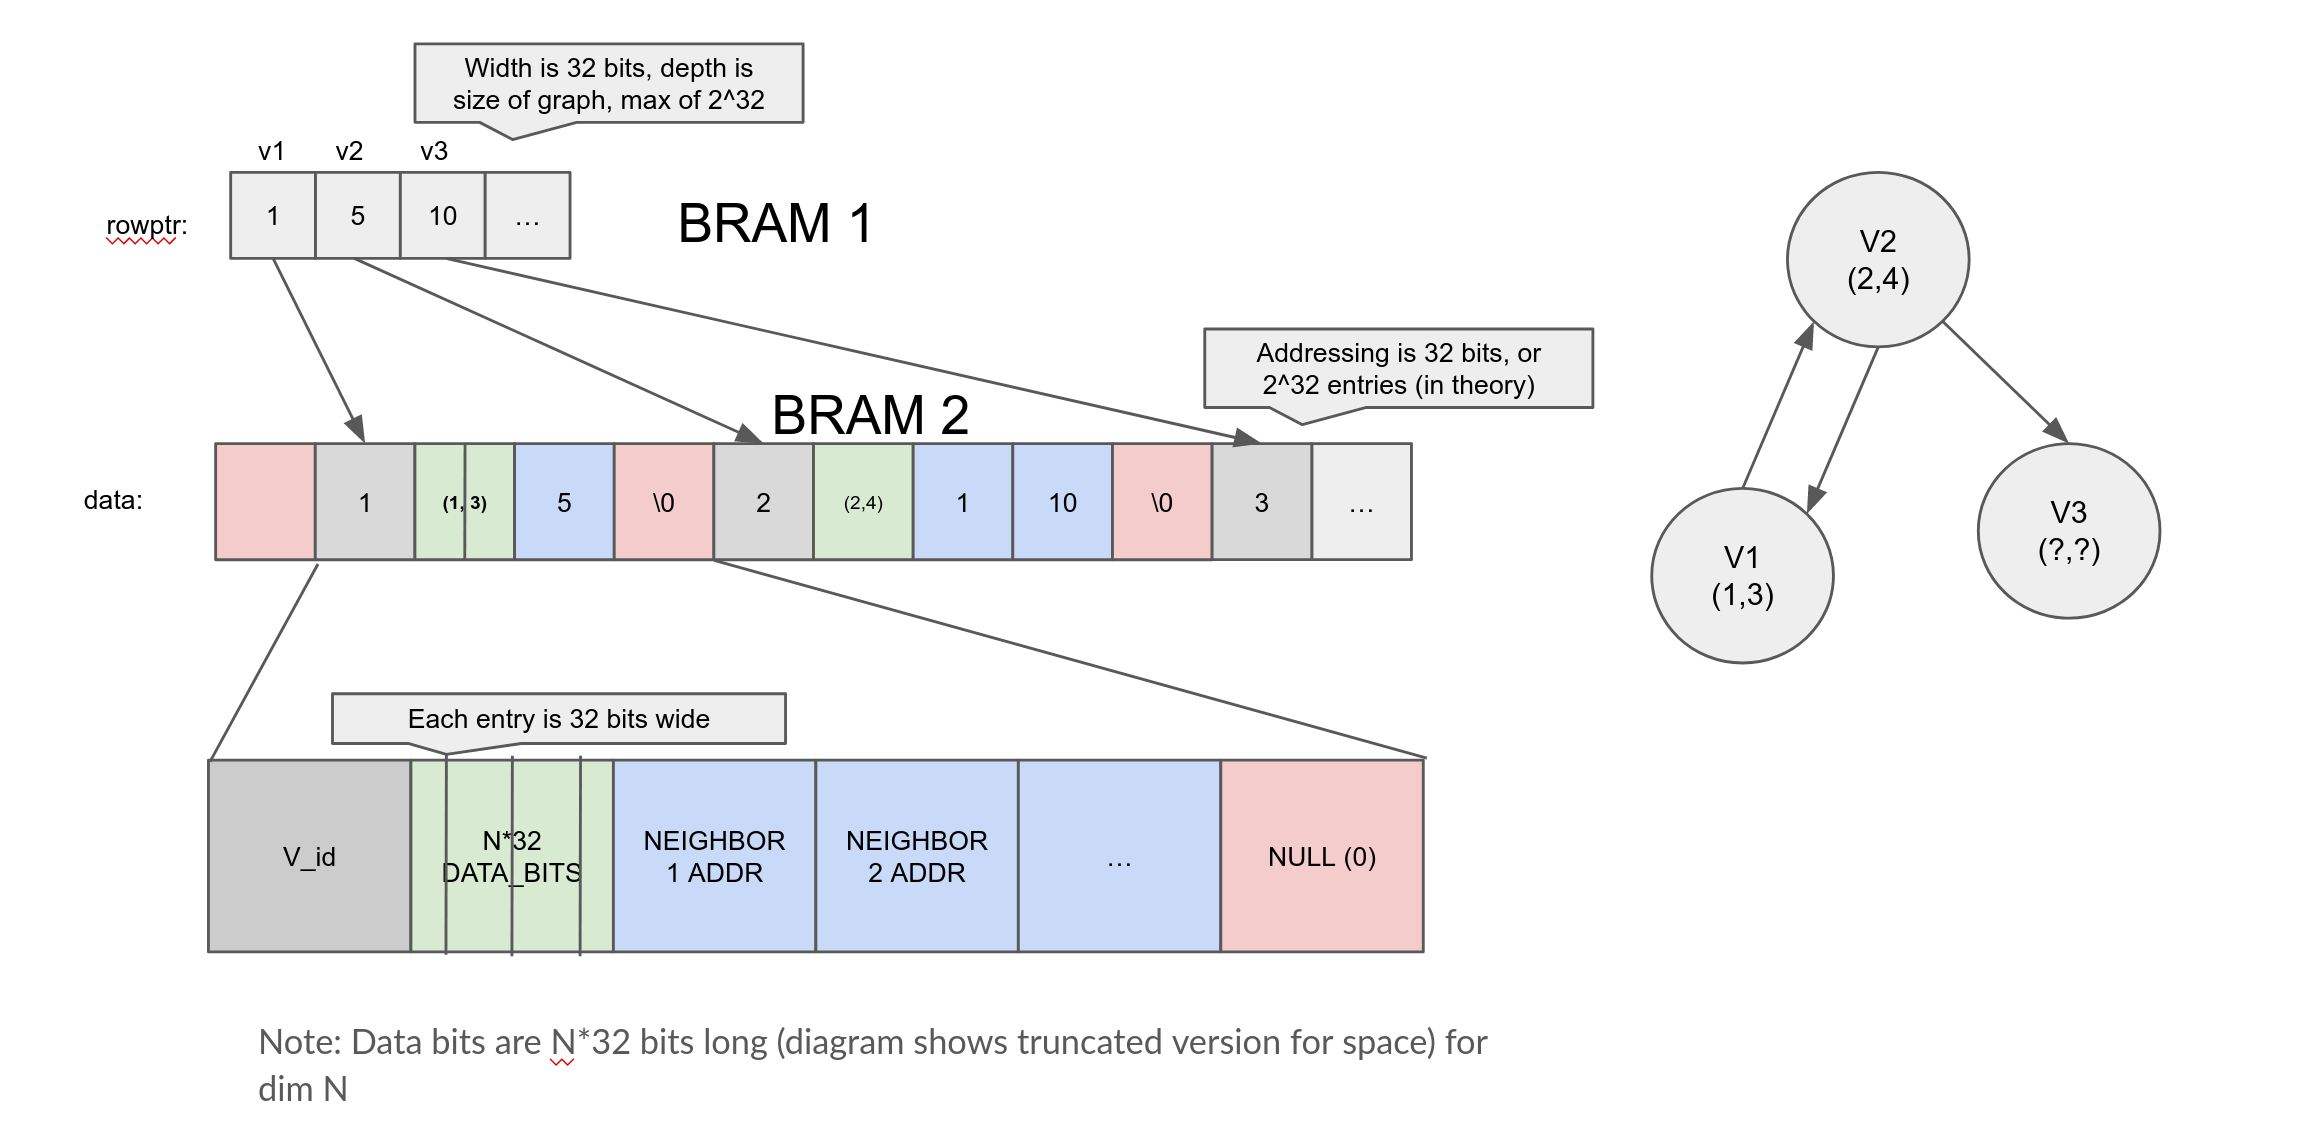
\includegraphics[width=9cm]{csr.png}}
\caption{Memory layout for graph storage}
\label{csrfig}
\end{figure}

BRAM 1 is a lookup table between vertex IDs and its associated address (ADDR) in the CSR data array. BRAM 2 has the position vector at ADDR+1 to ADDR+1+DIM and the neighbors from ADDR+2+DIM to the next 0 (NULL) value. BRAM 2 is dual port to allow two lookups at the same time.

\begin{lstlisting}[language=Verilog]
module graph_memory #(parameter DIM = 2, parameter PROC_BITS = 4)(
  input wire clk_in,
  input wire rst_in,
  input wire [31+PROC_BITS:0] idx_addr,
  input wire idx_validin,
  input wire [31+PROC_BITS:0] data_addra,
  input wire [31+PROC_BITS:0] data_addrb,
  input wire data_validina,
  input wire data_validinb,
  output logic [31:0] rowidx_out,
  output logic [31:0] data_outa,
  output logic [31:0] data_outb,
  output logic [31:0] data_outc,
  output logic data_valid_outa,
  output logic data_valid_outb,
  output logic rowidx_valid_out
  );    
\end{lstlisting}

We created a wrapper around the BRAM to maintain ordering and allow control signals, i.e. valid in and valid out. BRAMs are delayed two cycles, which is identified using control signals for appropriate buffering in a FIFO. The control signals are outputted using a state machine that returns a valid out two cycles after a valid input.

This memory is strictly read only. Currently, we operate on small graphs that can fit in BRAM alone.

To look up the address of some vertex ID, the memory abstraction provides a port to access the rowidx BRAM (single port) with a request for a certain ID. The result two cycles later is the ADDR corresponding to said ID.

\subsection{Graph Fetcher} \label{sssec:graphfetcher}

This module fetches [Figure \ref{fetchfig}] all graph data in order and buffers it for $n$ dimensions and an arbitrary number of neighbors. As aforementioned, the vertex location and the neighbor list are sequentially placed in memory. Given a certain vertex address (as computed from some vertex ID), we can iterate through the addresses to fetch the position vector and neighbors. 

% DIAGRAM HERE
\begin{figure}[htbp]
\centerline{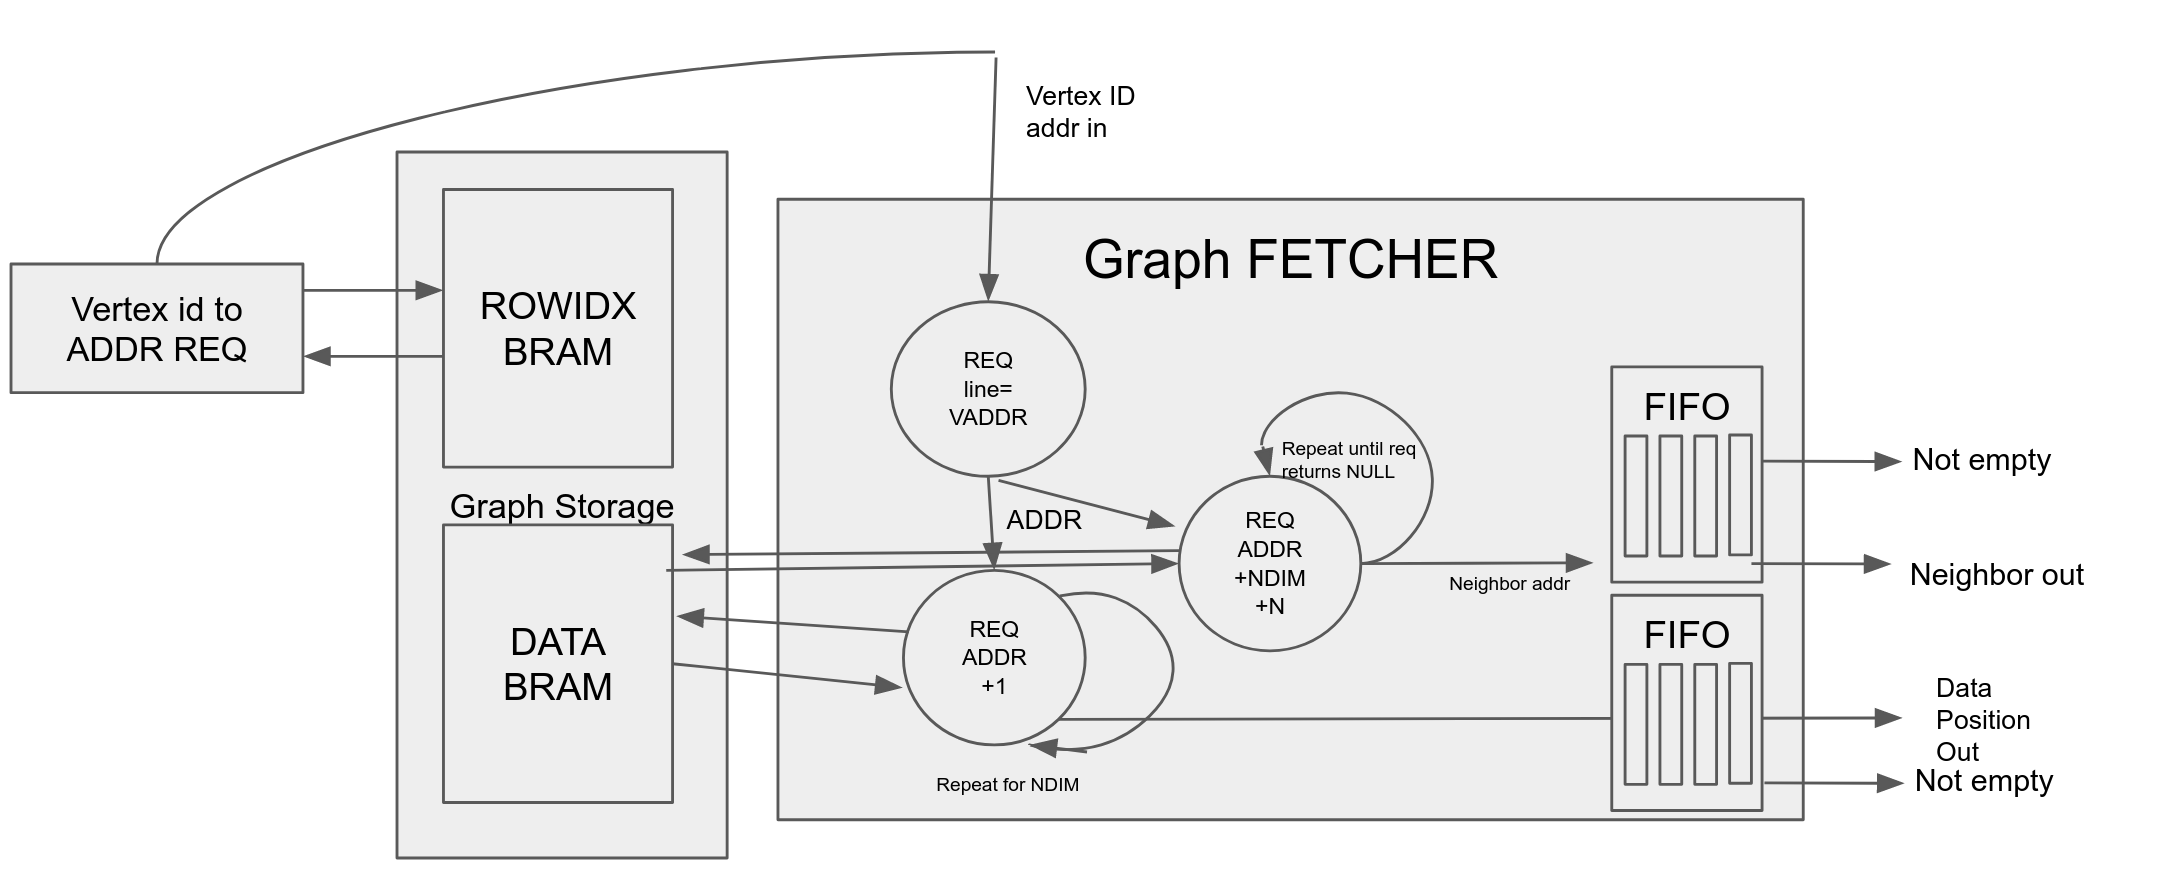
\includegraphics[width=9cm]{fetcher.png}}
\caption{Graph fetcher state machine.}
\label{fetchfig}
\end{figure}


This module starts by initializing the first position vector address at the vertex address + 1 and the first neighbor at vertex address + DIM + 1 and accessing the required data from the BRAM. We increment the request address at each step until we reach address + DIM + 1 for the position vector and value 0 (NULL) in the BRAM for the neighbors. We parallelize the lookup for neighbors and position by using the two ports on the BRAM. All outputs are buffered into two FIFOs (one for position and one for neighbors) to provide an easy access interface for other modules. Furthermore, the FIFOs allow caching of results when other modules are stalling/processing.

The fetching of the position vector and neighbors runs asynchronously. Specifically, after the data from the first  read request is received, we continue fetching the data at the subsequent address, storing the result in the corresponding FIFO queue to be read by the user until empty. For the position vector, the FIFO queue is size DIM since there will be at most DIM elements in the FIFO (assuming all elements are added before any are dequeued). The neighbor FIFO is fixed-size, and elements will be loaded only when space is available. If the FIFO is full before we read all neighbors, we stall the next neighbor BRAM request until an element has been dequeued from the neighbor FIFO. We will keep the FIFO around the average number of neighbors. The neighbor FIFO does not need to be emptied before starting to read the next vertex data since the order the neighbors will be visited remains the same. Note that while it is not depicted in the diagram for simplicity, each read request will include a delay of 2 cycles for BRAM to return, triggered by the ready bit on the memory module. FIFO reads, however, are single cycle. The neighbor and position vector FIFOs can dequeue/pop when data is ready/FIFO is not empty.

We tested our graph fetcher using a sample graph of 8 vertices with 4 dimensions each. Each vertex had between 2 and 4 neighbors, and most of the testing was completed with neighbor FIFO size greater than 4. Subsequent addresses for the position vector and neighbors were read every 3 cycles (2 cycles to receive data from the BRAM and 1 cycle to increment the address value once the received data was valid). This means that position vector fetching takes 3 * DIM cycles, and the neighbor fetching takes 3 * \# neighbors + 2 (must take 2 additional cycles to read 0 as the termination condition).

On the cycle that we increment the addresses, we also store the received values from the BRAM in their respective FIFOs. Our FIFOs were able to correctly dequeue the position vectors and neighbors in the order they were fetched. We also tested the module with neighbor FIFO size 2 on vertices with more than 2 neighbors. If the FIFO was full before all neighbors could be fetched, the module successfully stalled the BRAM requests until 1 of the neighbor FIFO elements could be dequeued.


\section{Incomplete Components}

\subsection{Message Router}
We expect multiple modules needing access to the memory, so we plan to make a module that will tag all memory requests with an ID for the requesting module. Memory results will retain this tag, associated by FIFO order on the requests. The message router will filter out the results for a given process for use there. A similar module will merge requests together to get sent to the memory module, supporting multiple requests per cycle and correctly distributing them.

\subsection{SPI Output}
We need to build the model that will dump the Priority Queue contents over SPI when complete. This should be largely unchanged from lab. We would use some microcontroller to handle the output.

\subsection{Large Graph Memory}

Ideally large graphs can be stored in DRAM, but that may not be finished by the end of the semester. Currently we assume graphs can fit in BRAM. Once we start working with larger graphs, we plan to have the BRAM used as a standard cache [Figure \ref{cachefig}] with the same interface that we currently use for requesting data. Since the class DRAM module may not be finished in time, we will use SPI to request an address and receive the result from the machine. This, again, can be reused  from lab. We would need to use a microcontroller to handle these connections.

\begin{figure}[htbp]
\centerline{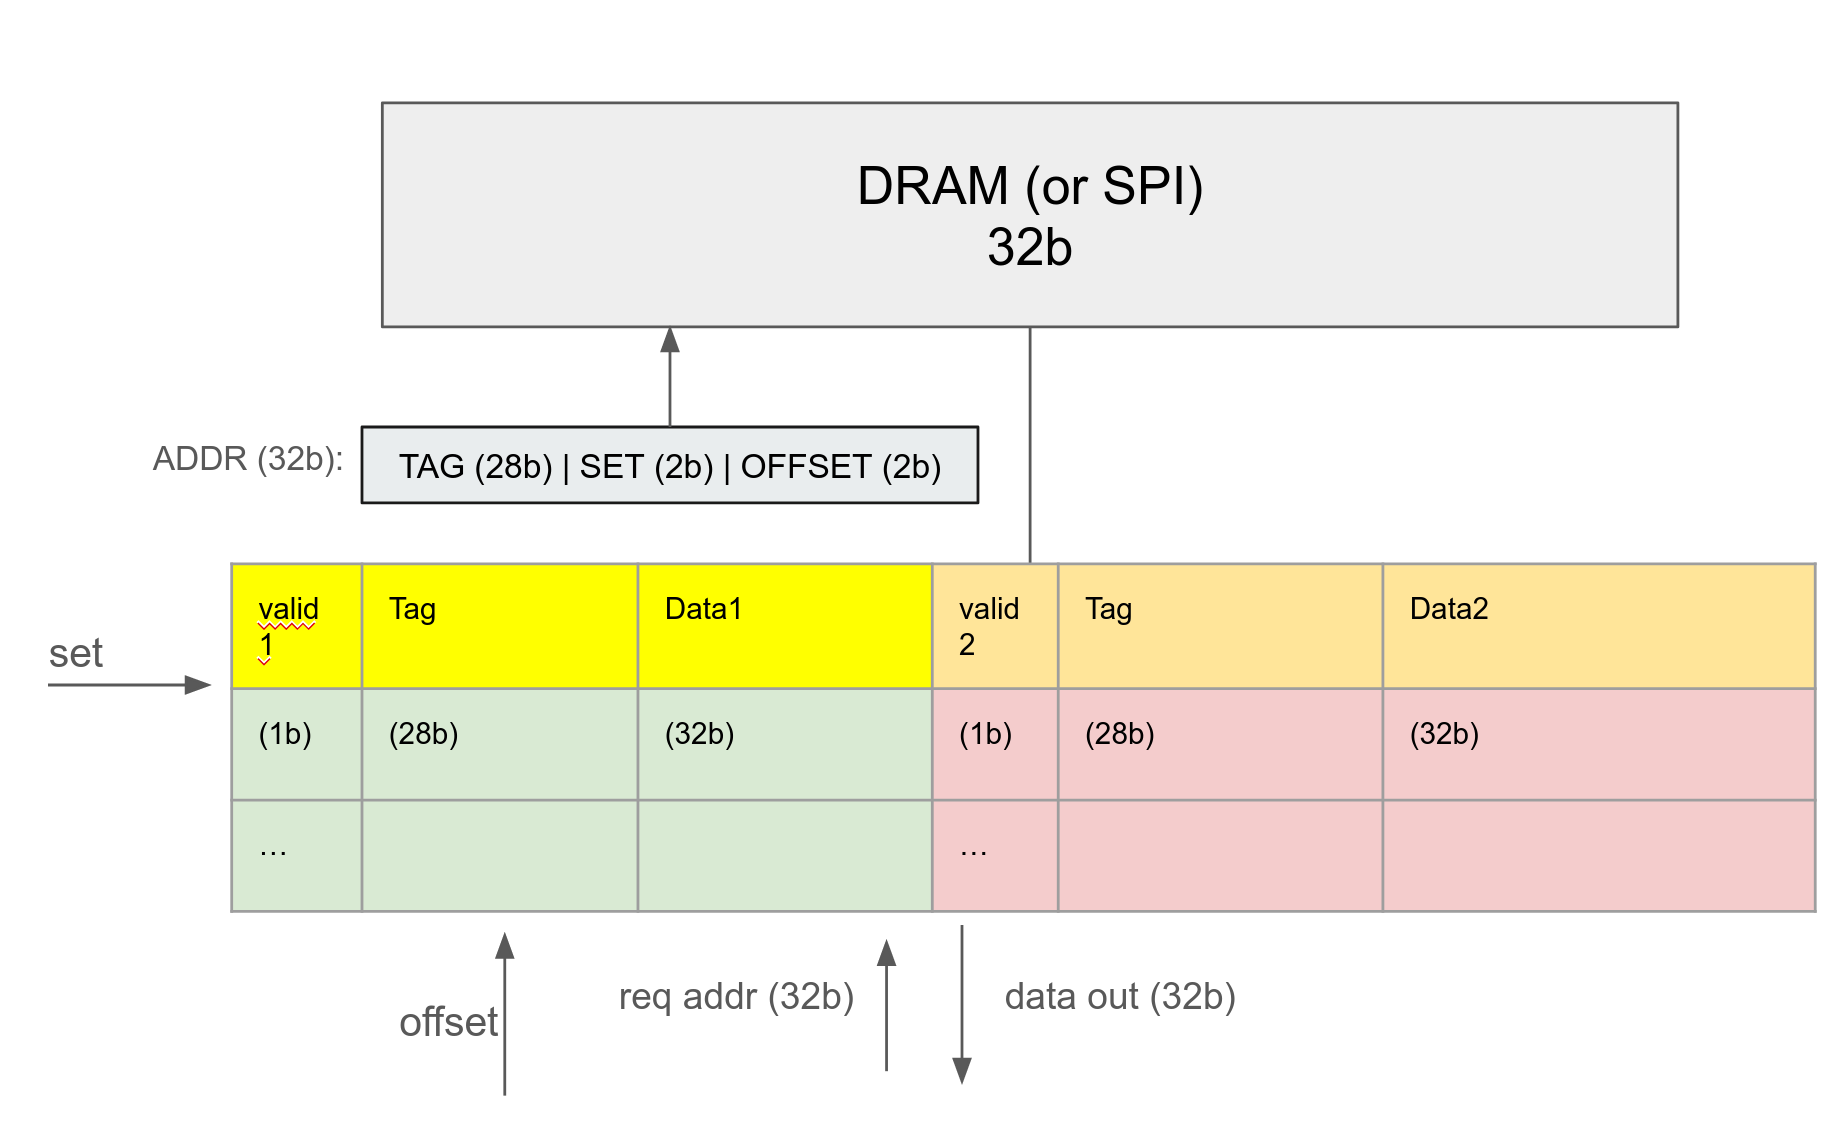
\includegraphics[width=8cm]{cache.png}}
\caption{DRAM/SPI based memory connected to a BRAM based cache. (dual port)}
\label{cachefig}
\end{figure}

\subsection{Checked/Visited BRAM}

We still need to create the BRAM to keep track of checked and visited vertices.

\subsection{Random Point Sampler}

Currently we choose the starting point as a hard-coded value. We will ideally use a pseudo-random sampler to find a better point closer to the destination (hard coded value).

At the moment, we see this module selecting a small random subset of vertices (possibly using an LFSR) from BRAM 1, computing the distances between each vertex and the query, and using the one with the smallest distance as the starting point. Choosing a starting point in this way would likely allow the algorithm to finish running in less iterations.

If we have time, this section will be implemented after the minimum viable product.

\subsection{Integration}

We need to connect all of the modules [\ref{fig:blockdiagram}] to actually implement BFiS. We are still planning on using a state machine for the BFiS algorithm, and the flow should be similar to the flow of our CPU code.

Modules will be connected as shown in the full block diagram. We will have it operating as a single threaded sequential machine to start. Time and space permitting, we should be able to add other workers via adding extra `cores', or multiple vector search instances.

\subsection{Synthesis on FPGA}

All of our verification so far has been in simulation, so we need to check that everything synthesizes correctly on the FPGA.

\section{Results \& Analysis}

We have tested everything made using custom testbenches in SystemVerilog. We have verified accuracy using a variety of inputs. Cycle analyses are written in prior sections when applicable.

% XXXX

\section{Conclusion}

We believe that the components we have implemented and plan to implement will effectively create an efficient graph-based vector search accelerator. We expect that our final system will produce better per-cycle results than CPU or GPU solutions based on a high degree of pipelining and parallelization of tasks. Our preliminary results from simulation are promising in creating a working final system. 


\section*{Acknowledgment}

We would like to thank Joe Steinmeyer and the 6.111 staff for their support and supervision during the course of this project's development. We would also like to thank Dr. Xuhao Chen and Prof. Arvind Mithal in the CSAIL Computation Structures Group who sponsored this project.

\bibliographystyle{IEEEtran}
\bibliography{IEEEabrv,IEEEexample}
% \printbibliography

\onecolumn\section{APPENDIX}

% Assortment of figures related to prior sections.



\subsection{C++ Code for CPU Implementing BFiS}\label{sssec:cpucode}

\begin{lstlisting}[language=C++]
#include <tuple> 
#include <queue>
#include "ann.h"
#include "utils.hh"
#include "common.hpp"

void kNN_search(int K, int qsize, int dim, size_t dsize, 
                const float *queries, const float *points, vid_t *results, Graph &g) {
   
  // find K closest points for each query
  for (int query_id=0; query_id<qsize; query_id++) {

      const float* query = queries + query_id * dim; // define query
      int L = 10*K; // queue capacity L
      int visited [dsize] = { 0 }; // create visited list
      

      // priority queues
      std::priority_queue<tuple<float,int>, vector<tuple<float, int>>, greater<tuple<float, int>>> S;
      std::priority_queue<tuple<float,int>> checked; 


      // index of starting point
      int index = 0;

      // distance calculation
      float dist = 0.0;
      for(int i=0; i< dim; i++){
        dist = dist + pow((points[i]-query[i]), 2);
      }
      dist = pow(dist, 0.5);


      // add starting point to S
      S.push(make_tuple(dist, index));
      visited[index] = 1;


      while (!S.empty()) {
        // first unchecked point
        vidType v = get<1>(S.top());

        // marked v_i as checked if less than L points checked or dist less than max checked dist
        if (checked.size() < L || get<0>(S.top()) < get<0>(checked.top())) {
          checked.push(S.top());

          // resize based on L  
          if (checked.size()>L) checked.pop();
        }
        
        // otherwise, if size is L, exit
        else {
          if(checked.size()==L) break;
        }
        S.pop();


        // iterate through neighbors
        for(vidType u:g.N(v)) {
          if (visited[u] == 0) {
            visited[u] = 1;


            // distance calculation
            const float* point = points + u*dim;
            dist = 0.0;
            for(int i=0; i< dim; i++){
              dist += pow(point[i]-query[i], 2);
            }
            dist = pow(dist, 0.5);


            // add point to S
            S.push(make_tuple(dist, u));
          }
        }
      }

      // remove elements not in top K
      while (checked.size() > K) {
        checked.pop();
      }

      // insert values in results
      int checked_length = checked.size();
      for (int i=0; (i<K && i<checked_length); i++) {
        results[query_id * K + (K-i-1)] = get<1>(checked.top());
        checked.pop();
      }
    }
}


\end{lstlisting}

% \begin{lstlisting}[language=C++]
%   for (int query_id=0; query_id<qsize; query_id++) {
%       const float* query = queries + query_id * dim;
%       int L = 10*K;
%       int visited [10000] = { 0 }; 
%       // priority queues vector and checked
%       std::priority_queue<tuple<float,int>, vector<tuple<float, int>>, greater<tuple<float, int>>> S;
%       std::priority_queue<tuple<float,int>> checked; 
%       ...
%       // distance calculation
%       float dist = 0.0;
%       for(int i=0; i< dim; i++){
%         dist = dist + pow((P_loc[i]-query[i]), 2);
%       }
%       dist = pow(dist, 0.5);
%       S.push(make_tuple(dist, index));
%       visited[index] = 1;
%       while (!S.empty()) {
%         vidType v = get<1>(S.top());
%         if (checked.size() < L || get<0>(S.top()) < get<0>(checked.top())) {
%           checked.push(S.top());

%           if (checked.size()>L) {
%             checked.pop();
%           }
%         }
%         else {
%           if(checked.size()==L) {
%             break;
%           }
%         }
%         S.pop();
%         // iterate through neighbors
%         for(vidType u:g.N(v)) {
%           if (visited[u] == 0) {
%             visited[u] = 1;
%             const float* point = points + u*dim; //points[u];
%             dist = 0.0;
%             for(int i=0; i< dim; i++){
%               dist += pow(point[i]-query[i], 2);
%             }
%             dist = pow(dist, 0.5);
%             S.push(make_tuple(dist, u));
%             // resize S based on L
%                 ....
%             }
%           }
%         }
%       }
%       while (checked.size() > K) {
%         checked.pop();
%       }
%         ....
%     }
% \end{lstlisting}

% Before you begin to format your paper, first write and save the content as a 
% separate text file. Complete all content and organizational editing before 
% formatting. Please note sections \ref{AA}--\ref{SCM} below for more information on 
% proofreading, spelling and grammar.

% Keep your text and graphic files separate until after the text has been 
% formatted and styled. Do not number text heads---{\LaTeX} will do that 
% for you.

% \subsection{Abbreviations and Acronyms}\label{AA}
% Define abbreviations and acronyms the first time they are used in the text, 
% even after they have been defined in the abstract. Abbreviations such as 
% IEEE, SI, MKS, CGS, ac, dc, and rms do not have to be defined. Do not use 
% abbreviations in the title or heads unless they are unavoidable.

% \subsection{Units}
% \begin{itemize}
% \item Use either SI (MKS) or CGS as primary units. (SI units are encouraged.) English units may be used as secondary units (in parentheses). An exception would be the use of English units as identifiers in trade, such as ``3.5-inch disk drive''.
% \item Avoid combining SI and CGS units, such as current in amperes and magnetic field in oersteds. This often leads to confusion because equations do not balance dimensionally. If you must use mixed units, clearly state the units for each quantity that you use in an equation.
% \item Do not mix complete spellings and abbreviations of units: ``Wb/m\textsuperscript{2}'' or ``webers per square meter'', not ``webers/m\textsuperscript{2}''. Spell out units when they appear in text: ``. . . a few henries'', not ``. . . a few H''.
% \item Use a zero before decimal points: ``0.25'', not ``.25''. Use ``cm\textsuperscript{3}'', not ``cc''.)
% \end{itemize}

% \subsection{Equations}
% Number equations consecutively. To make your 
% equations more compact, you may use the solidus (~/~), the exp function, or 
% appropriate exponents. Italicize Roman symbols for quantities and variables, 
% but not Greek symbols. Use a long dash rather than a hyphen for a minus 
% sign. Punctuate equations with commas or periods when they are part of a 
% sentence, as in:
% \begin{equation}
% a+b=\gamma\label{eq}
% \end{equation}

% Be sure that the 
% symbols in your equation have been defined before or immediately following 
% the equation. Use ``\eqref{eq}'', not ``Eq.~\eqref{eq}'' or ``equation \eqref{eq}'', except at 
% the beginning of a sentence: ``Equation \eqref{eq} is . . .''

% \subsection{\LaTeX-Specific Advice}

% Please use ``soft'' (e.g., \verb|\eqref{Eq}|) cross references instead
% of ``hard'' references (e.g., \verb|(1)|). That will make it possible
% to combine sections, add equations, or change the order of figures or
% citations without having to go through the file line by line.

% Please don't use the \verb|{eqnarray}| equation environment. Use
% \verb|{align}| or \verb|{IEEEeqnarray}| instead. The \verb|{eqnarray}|
% environment leaves unsightly spaces around relation symbols.

% Please note that the \verb|{subequations}| environment in {\LaTeX}
% will increment the main equation counter even when there are no
% equation numbers displayed. If you forget that, you might write an
% article in which the equation numbers skip from (17) to (20), causing
% the copy editors to wonder if you've discovered a new method of
% counting.

% {\BibTeX} does not work by magic. It doesn't get the bibliographic
% data from thin air but from .bib files. If you use {\BibTeX} to produce a
% bibliography you must send the .bib files. 

% {\LaTeX} can't read your mind. If you assign the same label to a
% subsubsection and a table, you might find that Table I has been cross
% referenced as Table IV-B3. 

% {\LaTeX} does not have precognitive abilities. If you put a
% \verb|\label| command before the command that updates the counter it's
% supposed to be using, the label will pick up the last counter to be
% cross referenced instead. In particular, a \verb|\label| command
% should not go before the caption of a figure or a table.

% Do not use \verb|\nonumber| inside the \verb|{array}| environment. It
% will not stop equation numbers inside \verb|{array}| (there won't be
% any anyway) and it might stop a wanted equation number in the
% surrounding equation.

% \subsection{Some Common Mistakes}\label{SCM}
% \begin{itemize}
% \item The word ``data'' is plural, not singular.
% \item The subscript for the permeability of vacuum $\mu_{0}$, and other common scientific constants, is zero with subscript formatting, not a lowercase letter ``o''.
% \item In American English, commas, semicolons, periods, question and exclamation marks are located within quotation marks only when a complete thought or name is cited, such as a title or full quotation. When quotation marks are used, instead of a bold or italic typeface, to highlight a word or phrase, punctuation should appear outside of the quotation marks. A parenthetical phrase or statement at the end of a sentence is punctuated outside of the closing parenthesis (like this). (A parenthetical sentence is punctuated within the parentheses.)
% \item A graph within a graph is an ``inset'', not an ``insert''. The word alternatively is preferred to the word ``alternately'' (unless you really mean something that alternates).
% \item Do not use the word ``essentially'' to mean ``approximately'' or ``effectively''.
% \item In your paper title, if the words ``that uses'' can accurately replace the word ``using'', capitalize the ``u''; if not, keep using lower-cased.
% \item Be aware of the different meanings of the homophones ``affect'' and ``effect'', ``complement'' and ``compliment'', ``discreet'' and ``discrete'', ``principal'' and ``principle''.
% \item Do not confuse ``imply'' and ``infer''.
% \item The prefix ``non'' is not a word; it should be joined to the word it modifies, usually without a hyphen.
% \item There is no period after the ``et'' in the Latin abbreviation ``et al.''.
% \item The abbreviation ``i.e.'' means ``that is'', and the abbreviation ``e.g.'' means ``for example''.
% \end{itemize}
% An excellent style manual for science writers is \cite{b7}.

% \subsection{Authors and Affiliations}
% \textbf{The class file is designed for, but not limited to, six authors.} A 
% minimum of one author is required for all conference articles. Author names 
% should be listed starting from left to right and then moving down to the 
% next line. This is the author sequence that will be used in future citations 
% and by indexing services. Names should not be listed in columns nor group by 
% affiliation. Please keep your affiliations as succinct as possible (for 
% example, do not differentiate among departments of the same organization).

% \subsection{Identify the Headings}
% Headings, or heads, are organizational devices that guide the reader through 
% your paper. There are two types: component heads and text heads.

% Component heads identify the different components of your paper and are not 
% topically subordinate to each other. Examples include Acknowledgments and 
% References and, for these, the correct style to use is ``Heading 5''. Use 
% ``figure caption'' for your Figure captions, and ``table head'' for your 
% table title. Run-in heads, such as ``Abstract'', will require you to apply a 
% style (in this case, italic) in addition to the style provided by the drop 
% down menu to differentiate the head from the text.

% Text heads organize the topics on a relational, hierarchical basis. For 
% example, the paper title is the primary text head because all subsequent 
% material relates and elaborates on this one topic. If there are two or more 
% sub-topics, the next level head (uppercase Roman numerals) should be used 
% and, conversely, if there are not at least two sub-topics, then no subheads 
% should be introduced.

% \subsection{Figures and Tables}
% \paragraph{Positioning Figures and Tables} Place figures and tables at the top and 
% bottom of columns. Avoid placing them in the middle of columns. Large 
% figures and tables may span across both columns. Figure captions should be 
% below the figures; table heads should appear above the tables. Insert 
% figures and tables after they are cited in the text. Use the abbreviation 
% ``Fig.~\ref{fig}'', even at the beginning of a sentence.

% \begin{table}[htbp]
% \caption{Table Type Styles}
% \begin{center}
% \begin{tabular}{|c|c|c|c|}
% \hline
% \textbf{Table}&\multicolumn{3}{|c|}{\textbf{Table Column Head}} \\
% \cline{2-4} 
% \textbf{Head} & \textbf{\textit{Table column subhead}}& \textbf{\textit{Subhead}}& \textbf{\textit{Subhead}} \\
% \hline
% copy& More table copy$^{\mathrm{a}}$& &  \\
% \hline
% \multicolumn{4}{l}{$^{\mathrm{a}}$Sample of a Table footnote.}
% \end{tabular}
% \label{tab1}
% \end{center}
% \end{table}

% \begin{figure}[htbp]
% \centerline{
\includegraphics{fig1.png}}
% \caption{Example of a figure caption.}
% \label{fig}
% \end{figure}



% Figure Labels: Use 8 point Times New Roman for Figure labels. Use words 
% rather than symbols or abbreviations when writing Figure axis labels to 
% avoid confusing the reader. As an example, write the quantity 
% ``Magnetization'', or ``Magnetization, M'', not just ``M''. If including 
% units in the label, present them within parentheses. Do not label axes only 
% with units. In the example, write ``Magnetization (A/m)'' or ``Magnetization 
% \{A[m(1)]\}'', not just ``A/m''. Do not label axes with a ratio of 
% quantities and units. For example, write ``Temperature (K)'', not 
% ``Temperature/K''.


% The preferred spelling of the word ``acknowledgment'' in America is without 
% an ``e'' after the ``g''. Avoid the stilted expression ``one of us (R. B. 
% G.) thanks $\ldots$''. Instead, try ``R. B. G. thanks$\ldots$''. Put sponsor 
% acknowledgments in the unnumbered footnote on the first page.

% \section*{References}

% Please number citations consecutively within brackets \cite{b1}. The 
% sentence punctuation follows the bracket \cite{b2}. Refer simply to the reference 
% number, as in \cite{b3}---do not use ``Ref. \cite{b3}'' or ``reference \cite{b3}'' except at 
% the beginning of a sentence: ``Reference \cite{b3} was the first $\ldots$''

% Number footnotes separately in superscripts. Place the actual footnote at 
% the bottom of the column in which it was cited. Do not put footnotes in the 
% abstract or reference list. Use letters for table footnotes.

% Unless there are six authors or more give all authors' names; do not use 
% ``et al.''. Papers that have not been published, even if they have been 
% submitted for publication, should be cited as ``unpublished'' \cite{b4}. Papers 
% that have been accepted for publication should be cited as ``in press'' \cite{b5}. 
% Capitalize only the first word in a paper title, except for proper nouns and 
% element symbols.

% For papers published in translation journals, please give the English 
% citation first, followed by the original foreign-language citation \cite{b6}.

% \bibliographystyle{ieeetran}
% % \bibliography{testing}

% \begin{thebibliography}{00}
% \bibitem{b1} Peng, Z., Zhang, M., Li, K., Jin, R., \& Ren, B. (2023, February). iQAN: Fast and Accurate Vector Search with Efficient Intra-Query Parallelism on Multi-Core Architectures. In Proceedings of the 28th ACM SIGPLAN Annual Symposium on Principles and Practice of Parallel Programming (pp. 313-328).
% % \bibitem{b2} J. Clerk Maxwell, A Treatise on Electricity and Magnetism, 3rd ed., vol. 2. Oxford: Clarendon, 1892, pp.68--73.
% % \bibitem{b3} I. S. Jacobs and C. P. Bean, ``Fine particles, thin films and exchange anisotropy,'' in Magnetism, vol. III, G. T. Rado and H. Suhl, Eds. New York: Academic, 1963, pp. 271--350.
% % \bibitem{b4} K. Elissa, ``Title of paper if known,'' unpublished.
% % \bibitem{b5} R. Nicole, ``Title of paper with only first word capitalized,'' J. Name Stand. Abbrev., in press.
% % \bibitem{b6} Y. Yorozu, M. Hirano, K. Oka, and Y. Tagawa, ``Electron spectroscopy studies on magneto-optical media and plastic substrate interface,'' IEEE Transl. J. Magn. Japan, vol. 2, pp. 740--741, August 1987 [Digests 9th Annual Conf. Magnetics Japan, p. 301, 1982].
% % \bibitem{b7} M. Young, The Technical Writer's Handbook. Mill Valley, CA: University Science, 1989.
% \end{thebibliography}
\vspace{12pt}
\color{red}
% IEEE conference templates contain guidance text for composing and formatting conference papers. Please ensure that all template text is removed from your conference paper prior to submission to the conference. Failure to remove the template text from your paper may result in your paper not being published.

\end{document}
